% !TEX encoding = UTF-8 Unicode
\documentclass[a4paper]{article}

% Dodato da se ne bi prikazivali podnaslovi u sadrzaju, a da ipak ostanu numerisani u okviru teksta
\setcounter{tocdepth}{1}    % levels under \subsection are not listed in the TOC


\usepackage{color}
\usepackage{url}
\usepackage[utf8]{inputenc} % make weird characters work
\usepackage{graphicx}


\usepackage[english,serbian]{babel}

\usepackage[unicode]{hyperref}
\hypersetup{colorlinks,citecolor=green,filecolor=green,linkcolor=blue,urlcolor=blue}

\usepackage{listings}

\newtheorem{primer}{Primer}[section]

\definecolor{mygreen}{rgb}{0,0.6,0}
\definecolor{mygray}{rgb}{0.7,0.7,0.7}
\definecolor{mymauve}{rgb}{0.58,0,0.82}

\lstset{ 
  backgroundcolor=\color{white},   % choose the background color; you must add \usepackage{color} or \usepackage{xcolor}; should come as last argument
  basicstyle=\scriptsize\ttfamily,        % the size of the fonts that are used for the code
  breakatwhitespace=false,         % sets if automatic breaks should only happen at whitespace
  breaklines=false,                 % sets automatic line breaking
  captionpos=b,                    % sets the caption-position to bottom
  commentstyle=\color{mygreen},    % comment style
  deletekeywords={...},            % if you want to delete keywords from the given language
  escapeinside={\%*}{*)},          % if you want to add LaTeX within your code
  extendedchars=true,              % lets you use non-ASCII characters; for 8-bits encodings only, does not work with UTF-8
%  firstnumber=1000,                % start line enumeration with line 1000
  frame=single,	                   % adds a frame around the code
  keepspaces=true,                 % keeps spaces in text, useful for keeping indentation of code (possibly needs columns=flexible)
  keywordstyle=\color{blue},       % keyword style
  language=SQL,                 % the language of the code
  morekeywords={*,...},            % if you want to add more keywords to the set
%  numbers=left,                    % where to put the line-numbers; possible values are (none, left, right)
%  numbersep=0pt,                   % how far the line-numbers are from the code
%  numberstyle=\tiny\color{mygray}, % the style that is used for the line-numbers
  rulecolor=\color{black},         % if not set, the frame-color may be changed on line-breaks within not-black text (e.g. comments (green here))
  showspaces=false,                % show spaces everywhere adding particular underscores; it overrides 'showstringspaces'
  showstringspaces=false,          % underline spaces within strings only
  showtabs=false,                  % show tabs within strings adding particular underscores
%  stepnumber=2,                    % the step between two line-numbers. If it's 1, each line will be numbered
  stringstyle=\color{mymauve},     % string literal style
  tabsize=2,	                   % sets default tabsize to 2 spaces
  title=\lstname                   % show the filename of files included with \lstinputlisting; also try caption instead of title
}

\renewcommand{\lstlistingname}{Kod}% Listing -> Algorithm
\renewcommand{\lstlistlistingname}{List of \lstlistingname s}%

\begin{document}

\title{Prepoznavanje saobraćajnih znakova koristeći CNN\\ \small{Seminarski rad u okviru kursa\\Računarska inteligencija\\ Matematički fakultet}}

\author{Jana Jovičić ???/2015, Jovana Pejkić 435/2016 \\ jana.jovicic755@gmail.com, jov4ana@gmail.com}

\date{16.~maj 2019.}

\maketitle

\abstract{

}

\newpage

\tableofcontents

\newpage

\section{Uvod}
\label{sec:uvod}



\section{Neuronske mreže}
\label{sec:cnn}

U masinskom ucenju, neuronske mreze (eng. neural networks) predstavljaju jednu od najprimenjenijih metoda. Neuronske mreže predstavljaju skup statističkih modela učenja inspirisana biološkim neuronima, za rešavanje klasifikacijskih i regresijskih problema. Njihove primene su mnogobrojne, a neke od njih su kategorijzacija teksta, medicinska dijagnostika, prepoznavanje objekata na slikama, autonomna voznja, igranje igara poput igara na tabli (tavla i go) ili video igara, masinsko prevodenje prirodnih jezika, modelovanje semantike reci prirodnog jezika i slicno. Problemi zahvaljujuci kojima su se neuronske mreze proslavile su velika kolicina podataka i ucenje na osnovu sirove reprezentacije podataka. Male kolicine podataka u slucaju neuronskih mreza lako vode preprilagodavanju, a ucenje nad do sada diskutovanim vektorskim reprezentacijama podataka ne koristi u dovoljnoj meri kljucnu prednost neuronskih mreza – da same konstruisu nove atribute nad sirovom reprezentacijom podataka. \footnote{Iako domenski eksperti nekad mogu pretpostaviti koji su atributi najinformativniji za predvidanje ciljne promenljive, njihovi izbori nekada mogu biti i pogresni, a neretko losiji od onoga sto bi algoritam ucenja mogao da detektuje u sirovoj informaciji ako bi bio primenljiv na nju.}


\subsection{Arhitektura}

Osnovnu jedinicu gradje neuronske mreze predstavljaju neuroni, koji su medjusobno povezani vezama sa tezinama koje se podesavaju tokom učenja mreže. Povezani neuroni prosledjuju signale jedni drugima, a organizovani su u slojeve. Najjednostavniji oblik neuronske mreze je perceptron, koji sadrzi samo jedan ulazni i jedan izlazni sloj. Medjutim, kako on sluzi samo za ucenje linearnih modela, a u praksi se javlja potreba da i slozeniji modeli mogu da se nauce, osim perceptrona, koriste se viseslojne neuronske mreze. Viseslojna neuronska mreza osim ulaznog i izlaznog sloja, dodatno ima jedan ili vise skrivenih slojeva. Broj skrivenih slojeva je proizvoljan, dok sama struktura skrivenog sloja utiče na performanse mreže. Kako se neuronske mreze uglavnom koriste za klasifikaciju uzorka u razlicite kategorije, ulazni sloj se sastoji od onoliko neurona kolika je dimenzionalnost ulaznog prostora, a broj neurona na izlazu jednak je broju klasa. Samo učenje neuronske mreže je zapravo podešavanje težina sve dok se ne dobije zadovoljavajuća aproksimacija između ulaznih i izlaznih veličina.

% TODO: Namestiti da slika bude unutar poglavlja 2.2 Prepoznavanje!

\begin{figure}[h!]
\begin{center}
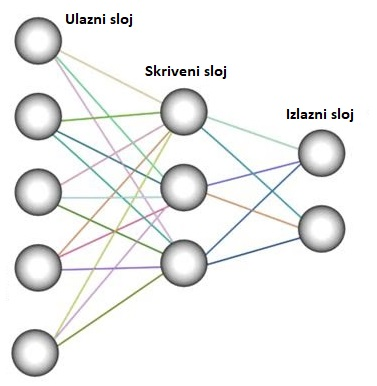
\includegraphics[scale=1]{neural_network_layers.jpeg}
\end{center}
\caption{Višeslojna neuronska mreža sa jednim skrivenim slojem}
\label{fig:neural_network_layers}
\end{figure}



\subsection{Prepoznavanje}

Jednostavni zadaci prepoznavanja mogu se dosta dobro rešiti skupovima podataka malih veličina, na primer desetine hiljada slika. Međutim, objekti u realističnim postavkama pokazuju značajnu varijabilnost, stoga, da bi bilo moguce naučiti prepoznati ih, potrebno je koristiti mnogo veće skupove za treniranje. Da bismo naučili o hiljadama objekata iz miliona slika, potreban nam je model sa velikim kapacitetom učenja. Konvolutivne neuronske mreže (CNN), koje ce biti detaljno obradjene u ostatku rada, čine jednu takvu klasu modela. Njihov kapacitet se moze kontrolisati variranjem njihove dubine i širine, a oni takođe daju jake i uglavnom ispravne pretpostavke o prirodi slika (naime, stacionarnost statistike i lokalitet zavisnosti piksela). Tako, u poređenju sa standardnim (feedforward) neuronskim mrežama sa slojevima sličnih veličina, CNN imaju mnogo manje veza i parametara, tako da ih je lakše trenirati, dok je njihov teoretski-najbolji učinak verovatno samo nešto lošiji.



\section{Konvolutivne neuronske mreže}	
\label{sec:podnaslov3}

%\cite{ime_knjige}.

Konvolutivne neuronske mreze predstavljaju podklasu neuronskih mreza koja ima najmanje jedan konvolutivni sloj (a moze ih imati i vise). Ova vrsta neuronskih mreza je inspirisana vizuelnim korteksom. Svaki put kada nešto vidimo, aktivira se niz slojeva neurona, i svaki sloj otkriva skup karakteristika kao što su linije, ivice. Visi nivoi slojeva otkritivaju složenije karakteristike kako bi prepoznali ono što smo videli. Konvolutivne mreze rade po istom principu i prakticno su uvek duboke neuronske mreze, upravo zbog toga sto je potrebno od sitnijih detalja, poput uspravnih, kosih i horizontalnih linija, koji obicno bivaju detektovani u nizim slojevima mreze, iskonstruisati slozenije oblike poput delova lica. Konvolutivne neuronske mreze se koriste u obradi signala (slike, zvuka), ali i teksta. U odnosu na ostale vrste neuronskih mreza, isticu se u prikupljanju lokalnih informacija (na primer o susednim pikselima na slici ili surrounding recima u tekstu) i smanjenju slozenosti modela (faster training, needs fewer samples, reduces the chance of overfitting). Konvulativne neuronske mreze se zasnivaju na sposobnosti mreza da iz sirovog signala konstruisu atribute. Nazivaju se konvolutivnim zato sto uce filtere, cijom konvolutivnom primenom detektuju odredena svojstva signala.

Unutrasnja struktura konvolutivne mreže se sastoji od nekoliko naizmeničnih konvolutivnih slojeva (eng. convolution layer) i slojeva agregacije (eng. pooling layer), pri cemu je dozvoljeno pojavljivanje iste vrste sloja vise puta. U dosad opisanoj strukturi neurona (neuronskih mreza) izlaz iz svakog od njih je bio skalarna veličina. Izlazi konvolutivnog sloja su dvodimenzionalni i nazivaju se mapama karakteristika (engl. feature maps). Izlazi konvolutivnog sloja se transformisu nelinearnom aktivacionom funkcijom. Na izlaze poslednjeg od tih slojeva se obicno nadovezuje potpuno povezana mreza, koja uci nad atributima koje prethodni slojevi konstruisu (nekoliko potpuno povezanih slojeva koji su jednodimenzionalni).

\begin{figure}[h!]
\begin{center}
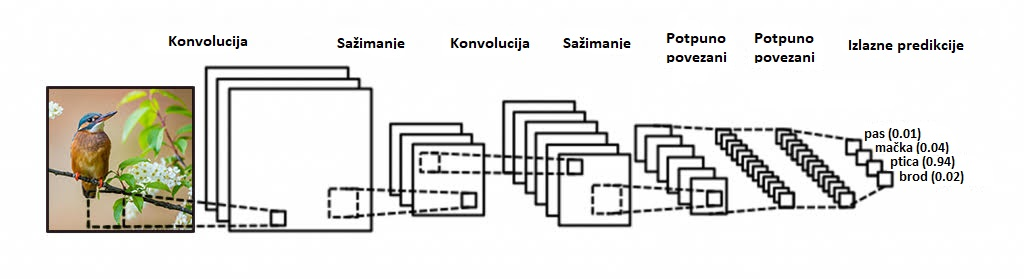
\includegraphics[scale=0.62]{cnn_layers.jpg}
\end{center}
\caption{Arhitektura konvolutivne neuronske mreže}
\label{fig:cnn_layers}
\end{figure}


\subsection{Konvolucija slika preko CNN}

%\ref{sec:ime_necega}.

Konvolutivne mreze primenjuju mnogo filtera nad jednom (jedinom) slikom, gde svaki prikuplja različite informacije. Na pocetnom sloju, mozete ih zamisliti kako prolazi filter za horizontalnu liniju, filter za vertikalnu liniju, i filter za dijagonalnu liniju da bi kreirali mapu ivica slike.

Konvulativne mreze uzimaju ove filtere, isecke prostora karakteristika slika, i mapiraju ih jednog po jednog; tj. oni kreiraju mapu gde beleže svako mesto gde se ta karakteristika javlja. Učeći razlicite delove prostora karakteristika, konvolutivne mreze dopustaju robusni inzenjering karakteristika. Konvulativne mreze uče slike iz delova koje zovemo mape karakteristika.

Konvolutivne mreze obavljaju neku vrstu pretrage. Zamislite malo uvelicavajuce staklo koje klizi s leva na desno preko vece slike, i nastavlja s leve strane kada dodje do kraja jednog prelaza (kao kod pisace masine). Taj pokretni (klizni) prozor moze da prepozna samo jednu stvar, recimo kratku vertikalnu liniju. Tri tamna piksela naslagana jedan na drugi?! Pomera taj filter za prepoznavanje (koji prepoznaje) vertikalnu liniju preko stvarnih piksela slike, trazeci podudaranja.

Svaki put kada se pronadje poklapanje (dodje do poklapanja), ono se mapira u (na) prostor sa karakteristikama koji je specifican za taj vizuelni element. U tom prostoru se cuva (belezi) lokacija svakog poklapanja sa vertikalnom linijom. Konvolutivna mreza pokrece mnogo, mnogo pretraga nad jednom slikom - horizontalne linije, dijagonalne linije, nad onoliko elemenata koliko se trazi (onoliko koliko ima vizuelnih elemenata koji trebaju da budu pretrazeni).

Nakon konvolutivnog sloja, ulaz se salje kroz nelinearnu transformaciju kao sto je tanh ili precišćena linearna jedinica?!, koja ce prevesti ulaz u opseg izmedju -1 i 1 (which will squash input values into a range between -1 and 1).


\begin{figure}[h!]
\begin{center}
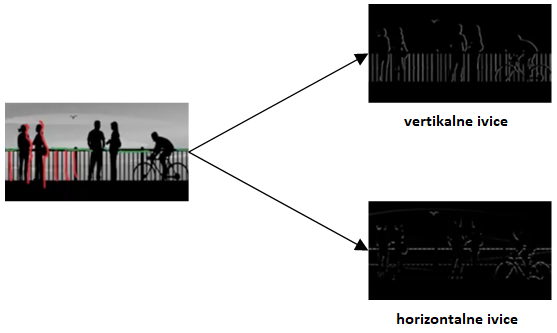
\includegraphics[scale=1]{edges.png}
\end{center}
\caption{Detektovanje ivica}
\label{fig:edges}
\end{figure}


\begin{figure}[h!]
\begin{center}
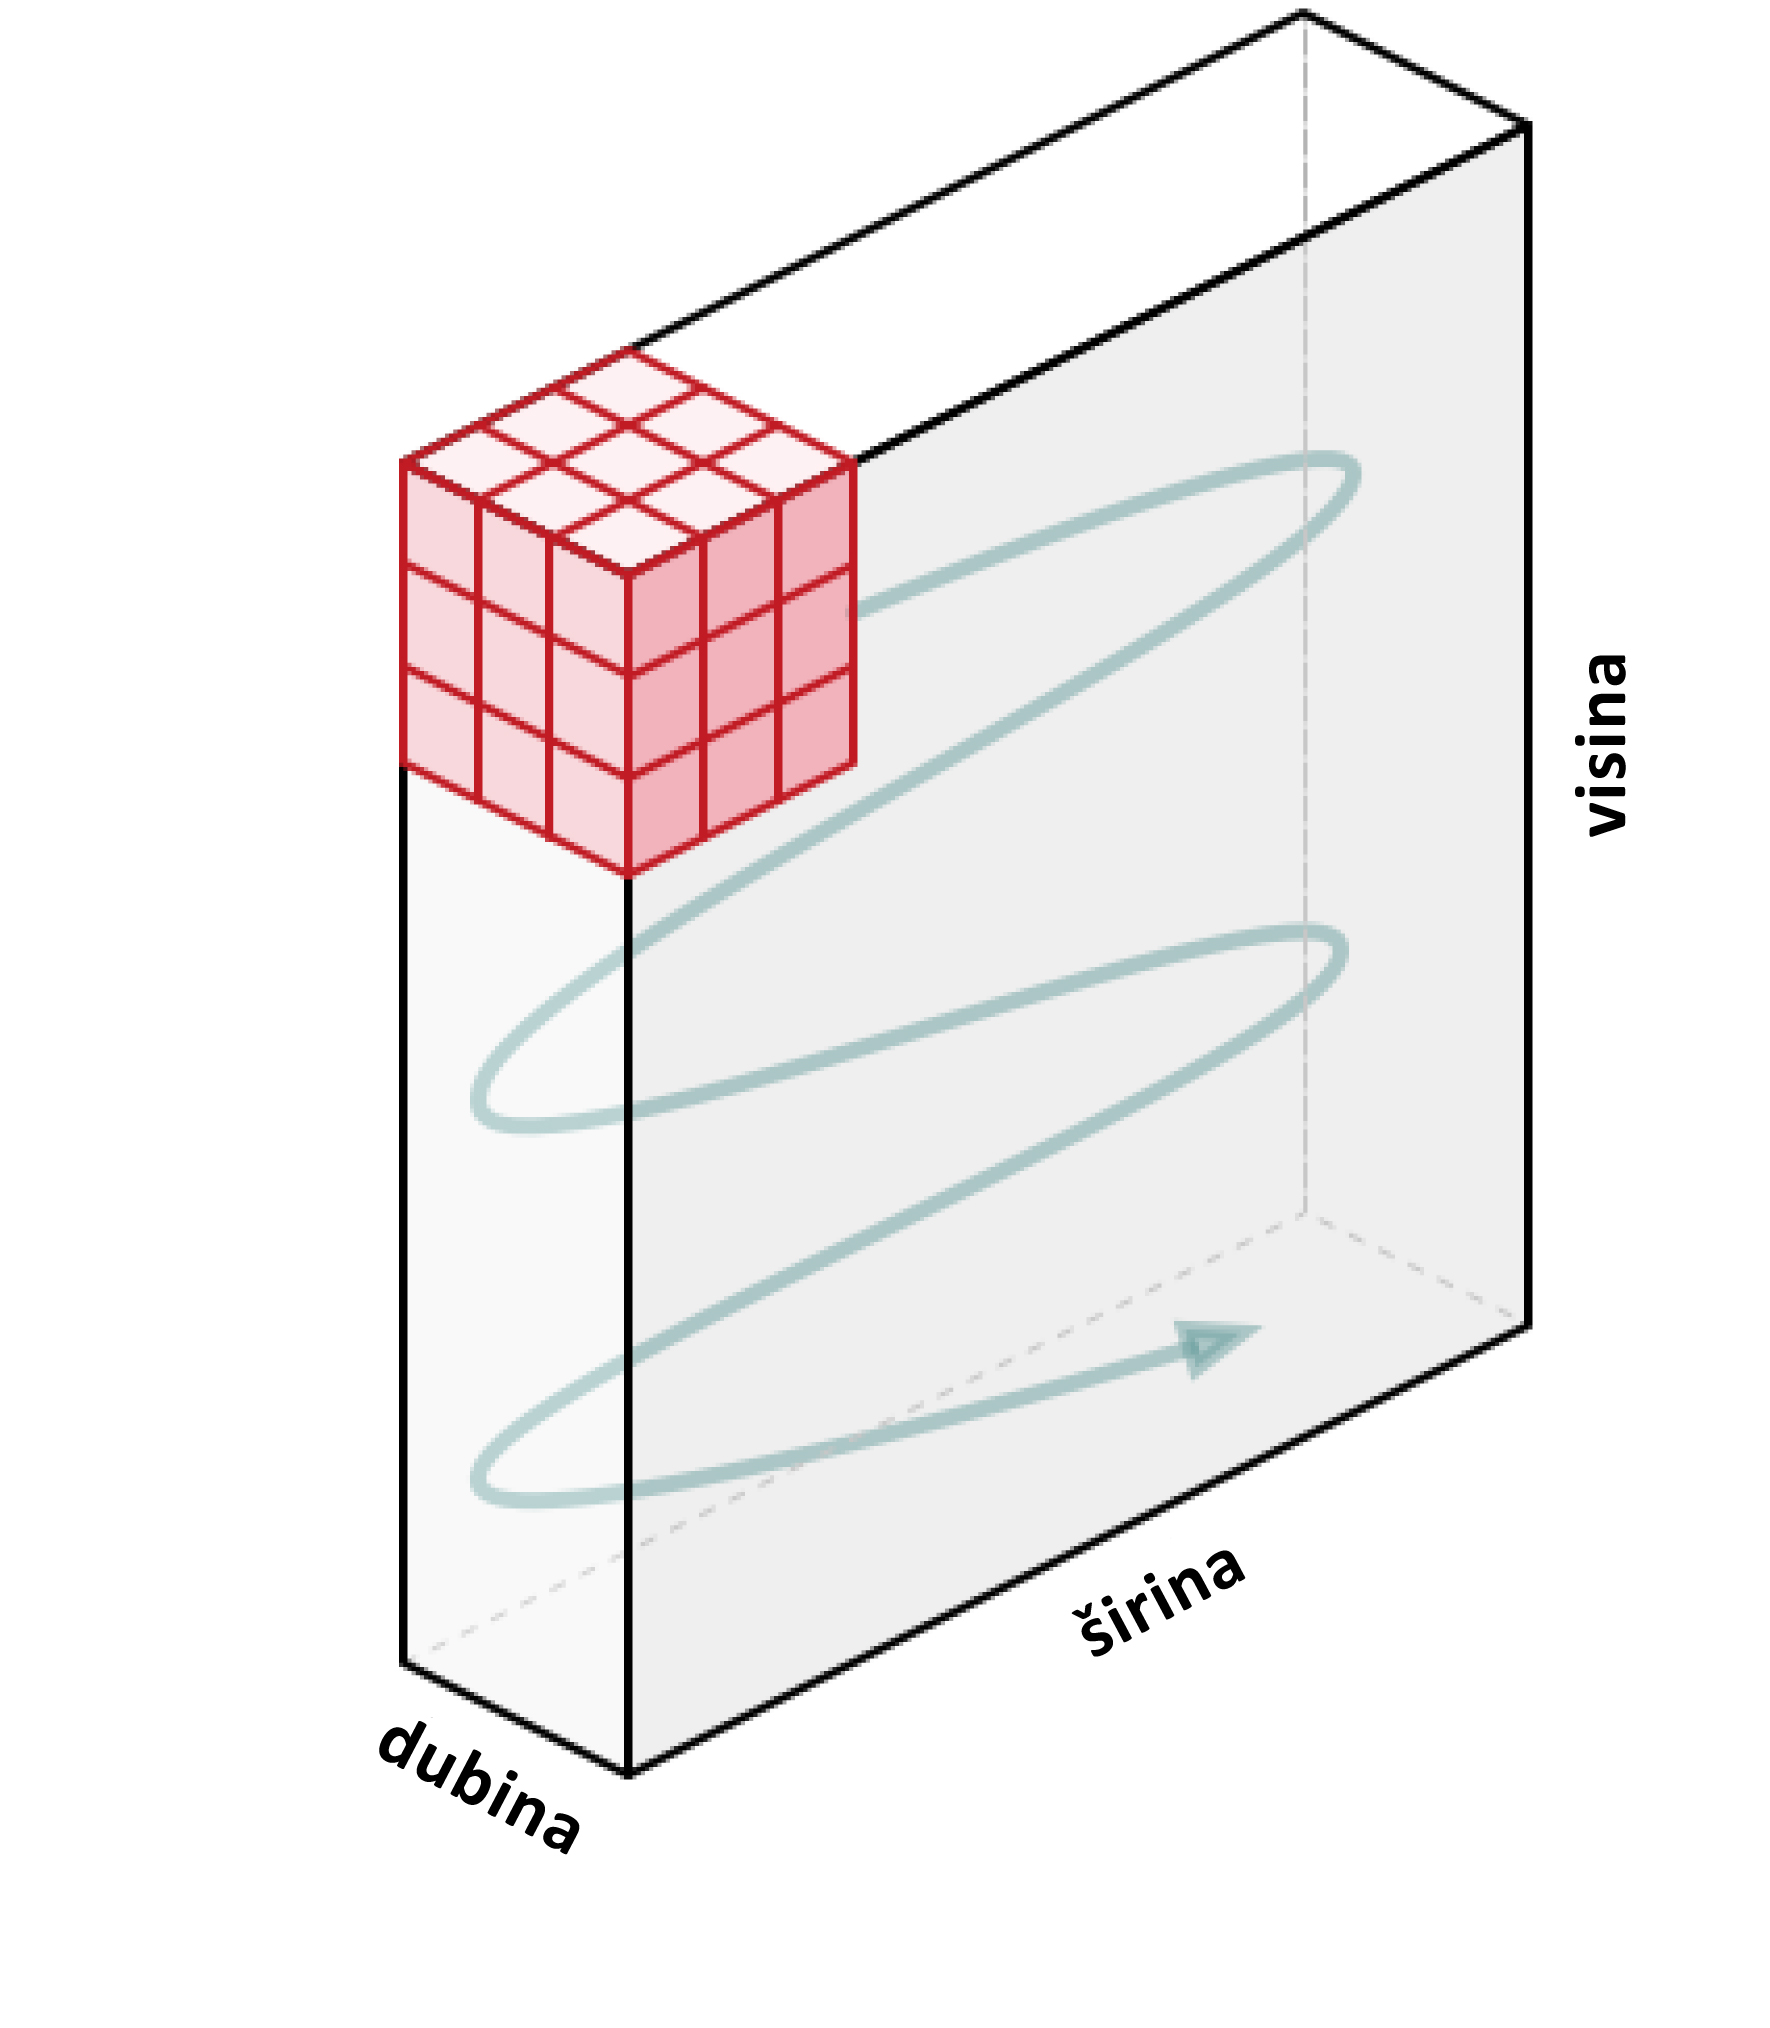
\includegraphics[scale=0.4]{filter_movement01.jpg}
\end{center}
\caption{Kretanje filtera}
\label{fig:filter_movement01}
\end{figure}



\begin{figure}[h!]
\begin{center}
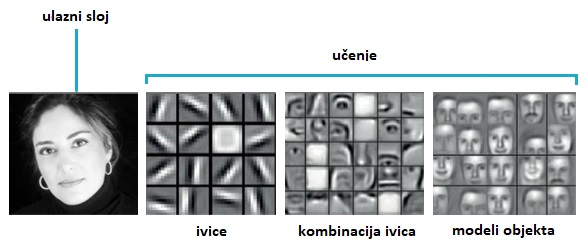
\includegraphics[scale=0.9]{learning.jpg}
\end{center}
\caption{Učenje mreže}
\label{fig:learning}
\end{figure}

\subsection{Konvolutivni sloj}

Konvolutivni sloj je glavni deo konvolutivne neuronske mreze. On radi najvise izracunavanja u mrezi, a ima ulogu konstrukcije novih atributa. To je prvi sloj koji ekstraktuje karakteristike iz ulazne slike. Konvolucija je matematicka operacija koja uzima dva ulaza - dve matrice f i g dimenzija m x n i p x q. Definisana je na sledeci nacin:
(f * g)ij = Xp minus 1 k=0 Xq minus 1 l=0 fi minus k,i minus lgk,l

Matrica f je obicno ulaz, poput slike, dok je matrica g filter (ili jezgro) – pomocna matrica koja izdvaja neku vrstu informacije iz ulaza. Određena ulazna reprezentacija podatka (originalna slika) konvolvira se s konvolucijskom jezgrom (filterom) s određenim parametrima. Procesom učenja ovi parametri (težine koje je potrebno nauciti kako bi mreža davala dobre rezultate) se podešavaju. Filteri su najcešce manjih prostornih dimenzija od ulaza, ali uvek su jednake dubine kao i ulaz. Konvolucijska jezgra (filteri) filtriraju sliku, tj. mapu karakteristika kako bi izlučila neku korisnu informaciju kao što je recimo određeni oblik, boja ili ivica. U prvih nekoliko slojeva izlučuju se osnovni oblici (npr. ivice). Jednostavan primer je filter za detekciju uspravnih ivica, horizontalnih ivica, dijagonalnih (kosih) ivica. Postojanje nekih objekata na slici se moze utvrditi na osnovu specificnog rasporeda ovih (uspravnih, kosih i horizontalnih) linija (ivica), koje detektuje prethodni konvolutivni sloj. Dalje, posmatra se kombinacija svih ovih ivica i tako prepoznaju i drugi oblici. Svaki konvolutivni sloj raspolaze nizom parametrizovanih filtera koji vrse ove poslove. Upravo, parametri filtera predstavljaju parametre konvolutivne mreze i bivaju nauceni u procesu obucavanja mreze.

Tokom prvog prolaza svaki filter se pomera po širini i visini i računa se skalarni proizvod ulaza i vrednosti filtera. Izlaz jednog filtera će biti dvodimenzioni niz. Ako imamo više filtera, izlaz iz konvolucionog sloja će biti rezultati svakog filtera poredjanih po dubini. Obično se koristi više konvolutivnih slojeva koji svojom kombinacijom mogu izučiti apstraktnije nivoe karakteristika karakteristične za pojedini objekt (npr. ljudsko lice). U zavisnosti od tipa filtera (jezgra) moguće je detektovati razne karakteristike (ivice, tačke). Vrednosti parametara jezgra se podešavaju procesom učenja tj. konvolucijske neuronske mreže na taj način „nauče“ prepoznavati određene karakteristike. Operacijom konvolucije dobija se transformirana slika I*K. Dobijena transformacija je lokalna tj. pikseli izlaza zavise o lokalnom susedstvu piksela ulaza.

\begin{figure}[h!]
\begin{center}
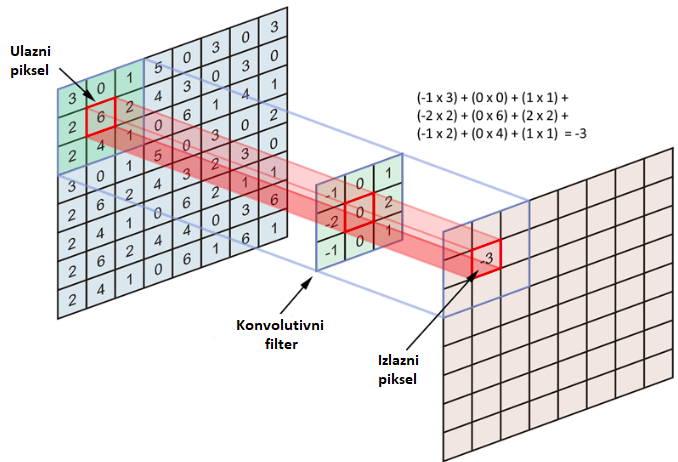
\includegraphics[scale=0.9]{convolution.png}
\end{center}
\caption{Konvolutivni sloj, pomeranje filtera}
\label{fig:convolution}
\end{figure}

\subsection{Prosirivanje}

Formula konvolucije koja je data iznad nije definisana za sve indekse i=0, m minus 1 i j=0, n minus 1.
 Na primer, ako je i, j = 0 i k, l > 0, vrednost fi minus k,i minus l nije definisana. Ukoliko bi se u obzir uzele samo definisane vrednosti, dimenzija konvolucije bi bila manja od dimenzije matrice f.
 
Medjutim, to nije uvek pozeljno, i moze se izbeci tako sto se vrsi prosirivanje (eng. padding) matrice f, na primer nulama ili vrednostima koje su vec na obodu, tako da velicina rezultujuce matrice bude jednaka velicini matrice f pre prosirivanja. Ovo je prikazano na slici ?????. Takode, prilikom racunanja konvolucije, filter se duz slike ne mora pomerati za jedan piksel, vec za neki veci korak (eng. stride).

\section{Sloj agregacije}
\label{sec:podnaslov5}

%\footnote{tekst koji se prikazuje kao fusnota}
%\textit{iskosen tekst}
%\ref{sec:primer_koda}

Uloga sloja za agregaciju je smanjenje broja parametara kada su slike prevelike, kao i smanjenje broja racunskih operacija u visim slojevima smanjuje. Agregacija smanjuje dimenzionalnost svake mape, ali zadržava važne informacije. Sve to rezultuje smanjenjem racunske zahtevnosti pri optimizaciji i pomaze u kontroli overfitinga. Zato zelimo da slojevi za agregaciju prate konvolucione slojeve kako bismo postepeno smanjili prostornu veličinu (širinu i visinu) prikaza podataka.

Cesto nas konačni zadatak postavlja neko globalno pitanje o slici, npr., Da li sadrži mačku? Tako da čvorovi našeg zadnjeg sloja moraju biti osetljivi na celi ulaz. Postepenom agregacijom informacija, stvarajuci grublje i grublje mape karakteristika, postize se taj cilj da se na kraju nauci globalna reprezentacija, zadrzavajuci sve prednosti konvolucijskih slojeva na srednjim slojevima obrade.

Sloj agregacije ukrupnjuje informacije, tako sto racuna neku jednostavnu funkciju agregacije susednih jedinica prethodnog sloja, poput maksimuma (eng. Max pooling) [koji vraca maksimalnu vrednost dela slike pokrivene filterom] ili proseka (eng. Average pooling) [koji vraca prosecnu vrednost dela slike pokrivene filterom]. Ukoliko agregira, na primer, 3 x 3 piskela, onda je broj izlaza ovog sloja 9 puta manji od broja izlaza prethodnog. Kada se racuna maksimum, dolazi do zanemarivanje informacije o tome gde je precizno neko svojstvo (poput uspravne linije) pronadeno, ali se ne gubi informacija da je pronadeno. Ovakva vrsta zanemarivanja informacije cesto ne steti cilju koji treba postici. Na primer, ako su na slici pronadeni kljun i krila, informacija o tacnoj pozicjiji najverovatnije nije bitna za odlucivanje da li se na slici nalazi ptica. Ipak, ukoliko je potrebno napraviti mrezu koja igra igru u kojoj su pozicije objekata na ekranu bitne, nije pozeljno koristiti agregaciju.

 Average pooling was often used historically but has recently fallen out of favor compared to the max pooling operation, which has been shown to work better in practice.
 
 Pooling layer downsamples the volume spatially, independently in each depth slice of the input volume.
 
Prva slika (pool): In this example, the input volume of size [224x224x64] is pooled with filter size 2, stride 2 into output volume of size [112x112x64]. Notice that the volume depth is preserved.
 
Druga slika (maxpool): The most common downsampling operation is max, giving rise to max pooling, here shown with a stride of 2. That is, each max is taken over 4 numbers (little 2x2 square).

 
\begin{figure}[h!]
\begin{center}
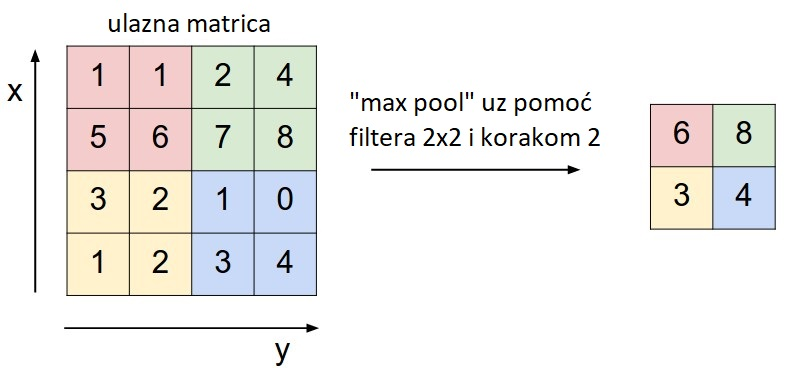
\includegraphics[scale=0.4]{maxpool.jpeg}
\end{center}
\caption{Maxpool}
\label{fig:maxpool}
\end{figure}


\begin{figure}[h!]
\begin{center}
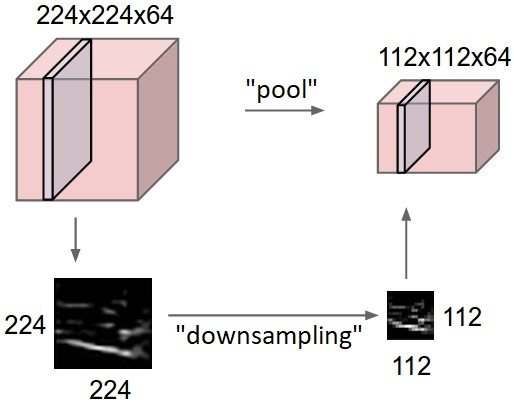
\includegraphics[scale=0.4]{pool.jpeg}
\end{center}
\caption{Pool}
\label{fig:pool}
\end{figure}


\begin{table}[h!]
\begin{center}
\caption{Primer tabele}
\begin{tabular}{|l|l|l|}
\hline
tekst & tekst & tekst tekst \\
\hline
tekst &  "tekst" &  tekst \\
\hline 
\end{tabular}
\label{tabela}
\end{center}
\end{table}

\subsection{Podnaslov 6}
\label{sec:podnaslov6}

Kod \ref{tabela1} demonstrira...

\begin{lstlisting}[caption={Primer koda},frame=single, label=tabela1]
table[key] = value
\end{lstlisting}


\subsection*{Podsekcija 1}


\subsubsection*{PodPodsekcija 1}


\subsection{Podnaslov 7}
\label{sec:podnaslov7}


\subsection{Podnaslov 8}
\label{sec:podnaslov8}


\section{Zaključak}
\label{sec:zakljucak}

\addcontentsline{toc}{section}{Literatura}
\appendix
\bibliography{seminarski} 
\bibliographystyle{plain}

\appendix
\section{Dodatak}
\subsection{Podnaslov 1}
%\label{sec:???}

\textbf{Dodatna objasnjenja} %TODO: Ubaciti u fusnote!


By visualizing the output from different convolution layers in this manner, the most crucial thing that you will notice is that the layers that are deeper in the network visualize more training data specific features, while the earlier layers tend to visualize general patterns like edges, texture, background etc.

This knowledge is very important when you use Transfer Learning whereby you train some part of a pre-trained network (pre-trained on a different dataset, like ImageNet in this case) on a completely different dataset. The general idea is to freeze the weights of earlier layers, because they will anyways learn the general features, and to only train the weights of deeper layers because these are the layers which are actually recognizing your objects.

Convolved Feature, Activation Map or Feature Map is the output volume formed by sliding the filter over the image and computing the dot product.
Perceptrons come first in 1950s, and it uses a brittle activation function to do classification, so if w*x is greater than some value it predicts positive, otherwise negative.

Neurons uses a softer activation function by introducing a sigmoid function, a tanh function or other activation functions to pass on values to other neurons in the network.

So perceptrons do not use in a network setting, they do classification on their own, hence they can’t classify XOR, however neurons can because they all contribute forward to the final output, using more complicated structure(i.e. multiple layers in network), they are able to classify XOR and other complicated problems.

A CNN, in specific, has one or more layers of convolution units. A convolution unit receives its input from multiple units from the previous layer which together create a proximity. Therefore, the input units (that form a small neighborhood) share their weights.

The convolution units (as well as pooling units) are especially beneficial as:

They reduce the number of units in the network (since they are many-to-one mappings). This means, there are fewer parameters to learn which reduces the chance of overfitting as the model would be less complex than a fully connected network.
They consider the context/shared information in the small neighborhoods. This future is very important in many applications such as image, video, text, and speech processing/mining as the neighboring inputs (eg pixels, frames, words, etc) usually carry related information.


\end{document}
